\documentclass[11pt, english]{article}              
        \usepackage{geometry}
                \geometry{                          
                        a4paper,total={210mm,297mm},
                        tmargin=40.8mm,
                        bmargin=40.8mm,
                        lmargin=32.6mm,
                        rmargin=32.6mm,
                }

        \usepackage{titlesec}         
                \titleformat{\section}
                        {\normalfont\fontsize{18}{16}\bfseries}{\thesection}{0.5em}{}
                \titleformat{\subsection}
                        {\normalfont\fontsize{14}{16}\bfseries}{\thesubsection}{1em}{}
                \titleformat{\subsubsection}
                        {\normalfont\fontsize{11}{16}\bfseries}{\thesubsubsection}{1em}{}

        \usepackage{longtable}
        \usepackage{multirow}

        \usepackage[labelfont=bf,textfont=bf,font=small,skip=8pt]{caption}

        \setlength{\parindent}{0pt}
        \renewcommand{\baselinestretch}{1.25}
       	\usepackage{setspace}

        \usepackage{amsmath}
        \usepackage{amssymb}

        \usepackage{tikz}
        	\usetikzlibrary{trees,arrows,topaths}

        \usepackage[utf8]{inputenc}
        \usepackage[official]{eurosym}

	\usepackage{float}

        \usepackage{graphicx}

\begin{document}

\pagenumbering{gobble}

        \title{\textsc{AG313 Treasury Management \& Derivatives\\ Coursework Examination}}
        \author{\textsc{Lewis Britton}}
        \date{\textsc{Academic Year 2019/2020}}
        \maketitle

\newpage

\pagenumbering{roman}

        \renewcommand{\contentsname}{Table of Contents}

        \tableofcontents 

\newpage

\pagenumbering{arabic}

\section{Investment Strategy}

	\subsection{Straddle (Question 1 (a))}

	\begin{table}[h]
		\scriptsize
		\renewcommand{\arraystretch}{1.25}
	\begin{center}
	\begin{tabular}{cccc}
		\hline
		\textbf{Share Price} & \textbf{Call Profit} & \textbf{Put Profit} & \textbf{Straddle Profit}\\
		\hline
		55 & -8 & 28 & 20\\
		65 & -8 & 18 & 10\\
		75 & -8 & 8 & 0\\
		\fbox{85} & -8 & -2 & -10\\
		95 & 2 & -2 & 0\\
		105 & 12 & -2 & 10\\
		115 & 22 & -2 & 20\\
		\hline
	\end{tabular}
	\end{center}
	\end{table}

	\begin{figure}[H]
	\begin{center}
		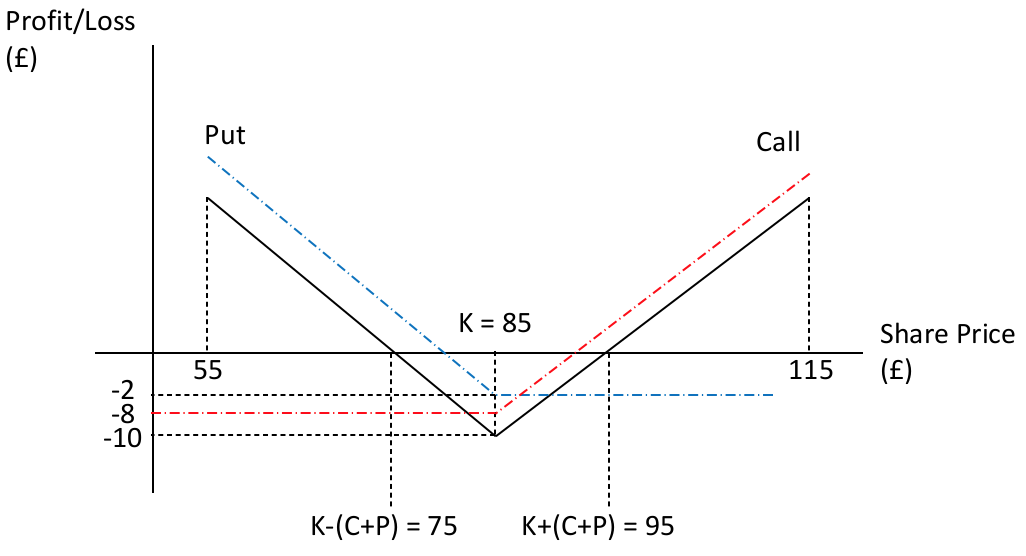
\includegraphics[height=5cm,width=10cm]{AG313-IMG/a.png}
	\end{center}
		\caption{Straddle Payoff}
	\end{figure}

	\subsection{Forward Rates (Question 1 (b))}

	$$F=S_0e^{rT}$$
	$$F=30e^{0.08(0.5)}$$
	$$31.2243\therefore\pounds31.22$$

	\begin{itemize}
	\setlength\itemsep{0cm}
		\item Enter a long-forward to buy oil in 6 months at the \pounds31 per barrel	
		\item Today, short-sell the oil for \pounds30 per barrel and invest the earnings at the risk-free rate to yield the equivalent of \pounds31.22 per barrel
		\item Close the short-sell after the 6 month period at the selling price of \pounds31 per barrel
		\item Leaves the profit of $\pounds31.22-\pounds31=\pounds0.22$
	\end{itemize}

	\subsection{Bull Spread (Question 1 (c))}

	\textit{Profit = Payoff from Long Call $+$ Payoff from Short Call}

	$$\mathrm{For}\ S=45:\ (0-6)+(0+4)=-2\therefore \mathrm{Loss\ of}\ \pounds2$$
	$$\mathrm{For}\ S=55:\ ((55-50)-6)+(0+4)=3\therefore \mathrm{Profit\ of}\ \pounds3$$
	$$\mathrm{For}\ S=45:\ ((65-50)-6)+((65-50)+4)=8\therefore \mathrm{Profit\ of}\ \pounds8$$

	\begin{figure}[H]
        \begin{center}                                                  
                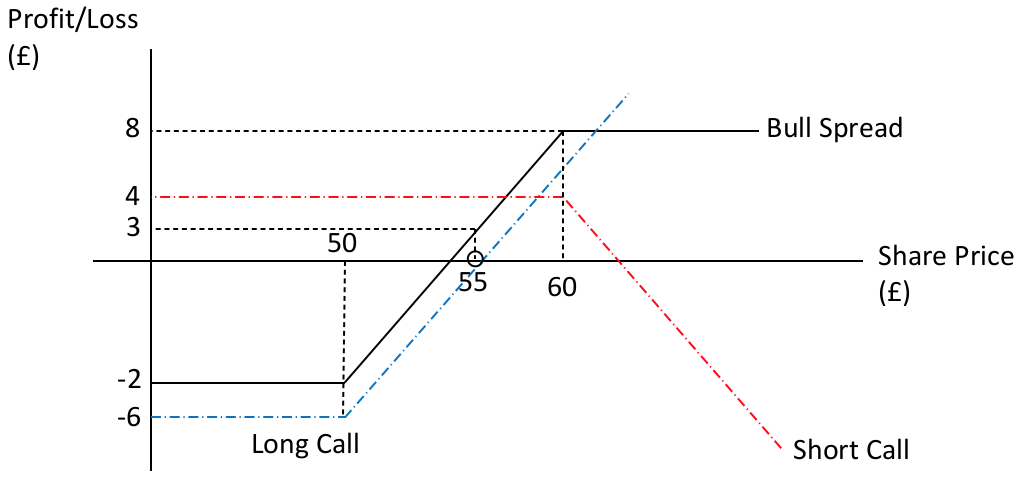
\includegraphics[height=5cm,width=10cm]{AG313-IMG/b.png}
        \end{center}              
                \caption{Bull Spread Payoff}
        \end{figure}

	\subsection{Interest Rate Swap (Question 1 (d))}

	\textit{Profit = Difference in Fixed $+$ Difference in Floating}

	$$0.015-((\mathrm{LIBOR}+0.006)-(\mathrm{LIBOR}+0.001))$$
	$$0.010\therefore1.00\%$$

	\begin{itemize}
	\setlength\itemsep{0cm}
		\item Therefore, 100 basis points 
		\item Bank recieve 0.2\% $\rightarrow$ 20 basis points
		\item X \& Y split 0.8\% $\rightarrow$ 80 basis points $\rightarrow$ 40 basis points ea.
		\item X's payoff: 0.065 $+$ 0.004 = 0.069 $\therefore$ 6.9\%
		\item Y's payoff: LIBOR $+$ 0.006 $+$0.004 = LIBOR $+$ 0.01 $\therefore$ LIBOR $+$ 1\%
		\item Bank's (intermediary's) payoff: 0.2\%
	\end{itemize}

	\begin{figure}[H]
	\begin{center}
		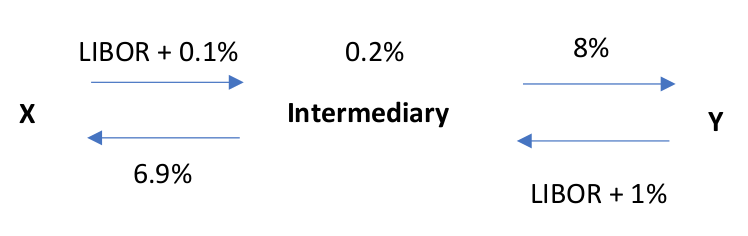
\includegraphics[height=3cm,width=10cm]{AG313-IMG/c.png}
	\end{center}
		\caption{Swap Structure}
	\end{figure}

\newpage

\section{Option Pricing}

	\subsection{Binomial Option Tree: European Put (Question (a))}

	\textbf{Step 1}

	$$u=e^{\sigma\sqrt{\Delta t}}=e^{0.30\sqrt{0.5}}=1.2363$$
	$$d=\frac{1}{u}=\frac{1}{1.2363}=0.8088$$
	$$p=\frac{e^{\sigma\sqrt{\Delta t}}}{u-d}=\frac{e^{0.30\sqrt{0.5}}}{1.2363-0.8088}=0.5672$$

	\textbf{Step 2}

	$$S_u=pu=10(1.2363)=12.363$$
	$$S_d=Pd=10(0.8088)=8.088$$
	$$S_{u,u}=Pu^2=10(1.2363)^2=15.284$$
	$$S_{u,d}=Pud=10\left((1.2363)(0.8088)\right)=9.999\approx10$$
	$$S_{d,d}=Pd^2=10(0.8088)^2=6.542$$

	\textbf{Step 3}

	$$P_{u,u}=0$$
	$$P_{u,d}=K-S_{u,d}=11-10=1$$
	$$P_{d,d}=K-S_{d,d}=11-6.542=4.458$$
	$$P_u=\left((pP_{u,u})+\left((1-p)P_{u,d}\right)\right)e^{-r\Delta t}=\left(((0.5672)0)+((1-0.5672)1)\right)e^{-0.1(0.5)}=0.412$$
	$$P_d=\left((pP_{u,d})+\left((1-p)P_{d,d}\right)\right)e^{-r\Delta t}=\left(((0.5672)1)+((1-0.5672)4.458)\right)e^{-0.1(0.5)}=2.375$$
	$$P_0=\left((pP_u)+\left((1-p)P_d\right)\right)e^{-r\Delta t}=\left(((0.5672)0.4117)+((1-0.5672)2.375)\right)e^{-0.1(0.5)}=1.199$$

	\newpage

	\textbf{Step 4}

	\tikzstyle{level 1}=[level distance=6cm, sibling distance=4cm]
        \tikzstyle{level 2}=[level distance=6cm, sibling distance=4cm]

        \tikzstyle{bag} = [text width=3em, text centered]
	\tikzstyle{end} = [text width=3em, text centered, inner sep=0pt]
	%[...minimum width=0pt, inner sep=0pt]

        \begin{tikzpicture}[grow=right, sloped]
                \node[bag] {10\\1.199}
                child {
                        node[bag] {8.088\\2.375} 
                        child {
				node[end] {6.542\\4.458}
				%node[end, label: {}]
                                edge from parent
					node[above] {}
					node[below] {}
                                }
                        child {
                                node[end] {10\\1}
                                edge from parent
                                        node[above] {}
                                        node[below] {}
                                }
                                edge from parent 
					node[above] {}
					node[below] {}
                        }
                child {
			node[bag] {12.363\\0.412}
                        child {
				node[end] {10\\1}
                                edge from parent
					node[above] {}
					node[below] {}
                                }
                        child {
                                node[end] {15.284\\0}
                                edge from parent
					node[above] {}
					node[below] {}
                                }
				edge from parent         
					node[above] {}
					node[below] {}
                        };
        \end{tikzpicture}

	\newpage

	\subsection{Binomial Option Tree: Converting to Americal Put (Question (b))}

	\textbf{Step 1}

	$$P_d=\max\{K-S_d,P_d\}$$
	$$P_d=\max\{11-8.088,2.375\}$$
	$$P_d=\max\{2.912,2.375\}$$
	$$2.912>2.375$$
	$$\therefore P_{d_A}=2.912$$

	\textbf{Step 2}

	$$P_{0_A}=((pP_{u_A})+((1-p)P_{d_A}))e^{-r\Delta t}=(((0.5672)0.4117)+$$
	$$((1-0.5672)2.912))e^{-0.1(0.5)}=1.421$$

	\textbf{Step 3}	

	\tikzstyle{level 1}=[level distance=6cm, sibling distance=4cm]
        \tikzstyle{level 2}=[level distance=6cm, sibling distance=4cm]

        \tikzstyle{bag} = [text width=3em, text centered]
        \tikzstyle{end} = [text width=3em, text centered, inner sep=0pt]

	\begin{tikzpicture}[grow=right, sloped]
                \node[bag] {10\\1.421}
                child {
                        node[bag] {8.088\\2.912} 
                        child {
                                node[end] {6.542\\4.458}
                                edge from parent
                                        node[above] {}
                                        node[below] {}
                                }
                        child {
                                node[end] {10\\1}       
                                edge from parent        
                                        node[above] {}
                                        node[below] {}
                                }                     
                                edge from parent      
                                        node[above] {}
                                        node[below] {}
                        }                             
                child {                               
                        node[bag] {12.363\\0.412}     
                        child {                       
                                node[end] {10\\1}     
                                edge from parent      
                                        node[above] {}
                                        node[below] {}
                                }                     
                        child {                       
                                node[end] {15.284\\0} 
                                edge from parent      
                                        node[above] {}
                                        node[below] {}
                                }                     
                                edge from parent      
                                        node[above] {}
                                        node[below] {}
                        };                            
        \end{tikzpicture}

	\newpage

	\subsection{Black \& Scholes Model (Question 2 (c))}

	\textbf{European Call}

	$$d_1=\frac{\ln\left(\frac{S}{K}\right)+T\left(r+\frac{\sigma^2}{2}\right)}{\sigma\sqrt{T}}=\frac{\ln\left(\frac{100}{110}\right)+\left(\frac{6}{12}\right)\left(0.06+\frac{0.30^2}{2}\right)}{0.30\sqrt{\frac{6}{12}}}=-0.202$$
	$$d_2=d_1-\sigma\sqrt{T}=-.202-0.30\left(\sqrt{\frac{6}{12}}\right)=0.414$$
	$$N(d_1)=0.4207;\ N(d_2)=0.3409$$
	$$C_0=SN(d_1)-Ke^{-rT}N(d_2)=5.6833$$
	$$\therefore\pounds5.68$$

	\textbf{American Call}

	$$C_{0_A}=C_{0_E}=5.6833$$
	$$\therefore\pounds5.68$$

	\textbf{European Put}

	$$P_0=(C_0+Ke^{-rT})-S=\left(5.6833+110e^{-0.06\left(\frac{6}{12}\right)}\right)-100=12.43$$
	$$\therefore\pounds12.43$$
	
	\textbf{Put-Call Parity Hold}\\

	Holds if: $(C_0+Ke^{-rT})=(P_0+S)$
	$$C_0+Ke^{-rT}=5.68+106.75=112.43$$
	$$P_0+S=12.43+100=112.43$$
	$$\therefore\ \mathrm{Parity Holds}$$

	\newpage

	\subsection{Portfolio Value (Question 2 (d))}

	$N$ short contracts to reduce risk by 0.25
	$$N=\Delta\sigma\beta_p\left(\frac{V_P}{V_F}\right)=(0.25)(1.1)\left(\frac{720\times10^6}{6110.8(10)}\right)=3240.165$$

	Profit of forward position at expiration
	$$(F_0-F_T)(10)(N)=(6110.8)(10)(3240.165)=-7873200$$
	$$\therefore\mathrm{Loss\ of\ }\pounds7,873,200$$

	In $t=3$ index $\Delta$'d by
	$$\frac{F_T-S}{S}=\frac{6353.8-6051.2}{6051.2}=0.050$$
	$$\therefore5.00\%$$

	Folio value expected to change by
	$$\Delta\beta_{Index}=0.05(1.1)=0.055$$
	$$\therefore5.5\%$$

	Value of folio at expiration
	$$V_P(1+E(\Delta V_P))=720\times10^6(1+0.055)=759605235.3$$
	$$\therefore\pounds759,605,235.30$$

	Folio: ($+$) 759605235.3\\
	Dividends: ($+$) 450000\\
	Futures: ($-$) 7873200\\
	$\therefore$ Total = 7531820353\\

	3-month return
	$$\frac{\mathrm{Total}-V_P}{V_P}=\frac{759605235.3-720\times10^6}{720\times10^6}=0.0461$$
	$$\therefore4.61\%$$

	Annualized return
	$$(1+3\ \mathrm{Month\ Return})^T-1=(1+0.0461)^{\frac{12}{3}}-1=0.1975$$
	$$\therefore19.75\%$$

\newpage

\section{Treasury Management}

	\subsection{Question 4 (a)}

	$$1000000(0.5116^{-1})=1954652.072$$
	$$\therefore\pounds1,954,652.07$$

	\subsection{Question 4 (b)}
	
	$$2000(0.6667^{-1})=2999.8500$$
	$$\therefore\pounds2999.85$$

	\subsection{Question 4 (c)}

	$$F_{180}=S_0e^{rT}=0.008058e^{0.0191\left(\frac{1}{2}\right)}=0.008135$$
	$$\therefore0.008135\frac{\$}{\yen}$$

	\subsection{Question 4 (d)}

	\begin{itemize}
	\setlength\itemsep{0cm}
		\item Buy \$10,000 at \textit{ask} rate
		\item $10000(1.631^{-1})=6131.2078$
		\item $\therefore\$6131.21$
		\item Resell at \textit{bid} rate
		\item $6131.2078(1.624)=9957.0815$
		\item $\therefore\$9957.08$
		\item $\therefore\mathrm{Cost\ of\ Transactions}=\$42.92$
	\end{itemize}

	\subsection{Question 4 (e)}

	$$\frac{\$}{\euro}=\frac{1}{\frac{\euro}{\$}}={\frac{\euro}{\$}}^{-1}=0.8^{-1}=1.25$$
	$$\therefore1.25\frac{\$}{\euro}$$

	\subsection{Question 4 (f)}

	$$p=\frac{1+0.05}{1+0.03}=1.0194$$
	$$F=1.5(1.0194)=1.5291$$
	$$\therefore1.5291\frac{\$}{\euro}$$

	\subsection{Question 4 (g)}

	\begin{itemize}
	\setlength\itemsep{0cm}
		\item Margin Call when $1000-500=1000$ is lost
		\item $62500\euro(1.5\$)=\$95,750$
		\item $93750-1000=92750\therefore\$92,750$
		\item Settlement price: $\frac{92750}{62500}=1.484\frac{\$}{\euro}\mathrm{req.}$
	\end{itemize}

\end{document}
